\documentclass[border=10pt]{standalone}
\usepackage{pgfplots}
\pgfplotsset{compat=1.18}
\begin{document}
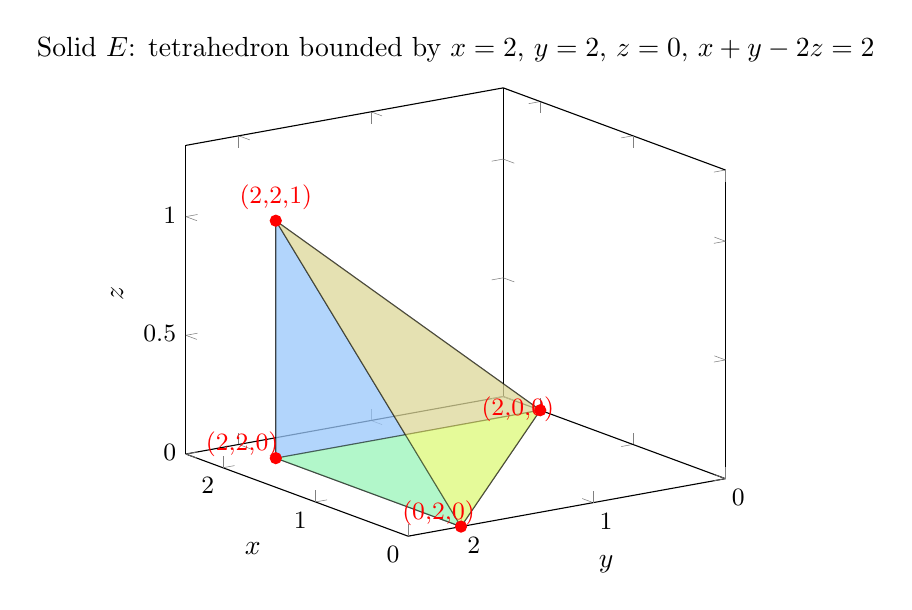
\begin{tikzpicture}
\begin{axis}[
    view={-125}{18},
    xlabel={$x$}, ylabel={$y$}, zlabel={$z$},
    xmin=0, xmax=2.4, ymin=0, ymax=2.4, zmin=0, zmax=1.3,
    tick label style={font=\small},
    title={Solid $E$: tetrahedron bounded by $x=2$, $y=2$, $z=0$, $x+y-2z=2$},
]
% Face x=2: vertices (2,2,0),(2,2,1),(2,0,0)
\addplot3[fill=blue!40, opacity=0.5, draw=black] coordinates {(2,2,0) (2,2,1) (2,0,0) (2,2,0)};
% Face y=2: vertices (2,2,0),(2,2,1),(0,2,0)
\addplot3[fill=cyan!40, opacity=0.5, draw=black] coordinates {(2,2,0) (2,2,1) (0,2,0) (2,2,0)};
% Face z=0: vertices (2,2,0),(2,0,0),(0,2,0)
\addplot3[fill=green!40, opacity=0.5, draw=black] coordinates {(2,2,0) (2,0,0) (0,2,0) (2,2,0)};
% Face x+y-2z=2: vertices (2,2,1),(2,0,0),(0,2,0)
\addplot3[fill=yellow!60, opacity=0.5, draw=black] coordinates {(2,2,1) (2,0,0) (0,2,0) (2,2,1)};
% Vertex (2,2,1)
\addplot3[only marks, mark=*, mark size=2pt, color=red] coordinates {(2,2,1)};
\node[red, font=\small] at (axis cs:2,2,1.1) {(2,2,1)};
% Vertex (2,0,0)
\addplot3[only marks, mark=*, mark size=2pt, color=red] coordinates {(2,0,0)};
\node[red, font=\small] at (axis cs:2.1,0.1,0) {(2,0,0)};
% Vertex (0,2,0)
\addplot3[only marks, mark=*, mark size=2pt, color=red] coordinates {(0,2,0)};
\node[red, font=\small] at (axis cs:0.1,2.1,0.05) {(0,2,0)};
% Vertex (2,2,0)
\addplot3[only marks, mark=*, mark size=2pt, color=red] coordinates {(2,2,0)};
\node[red, font=\small] at (axis cs:2.15,2.15,0.05) {(2,2,0)};
\end{axis}
\end{tikzpicture}
\end{document}